% Charge Computing Framework Figure Captions
% Categorical State Propagation in Electrical Systems

\begin{figure*}[!htbp]
\centering
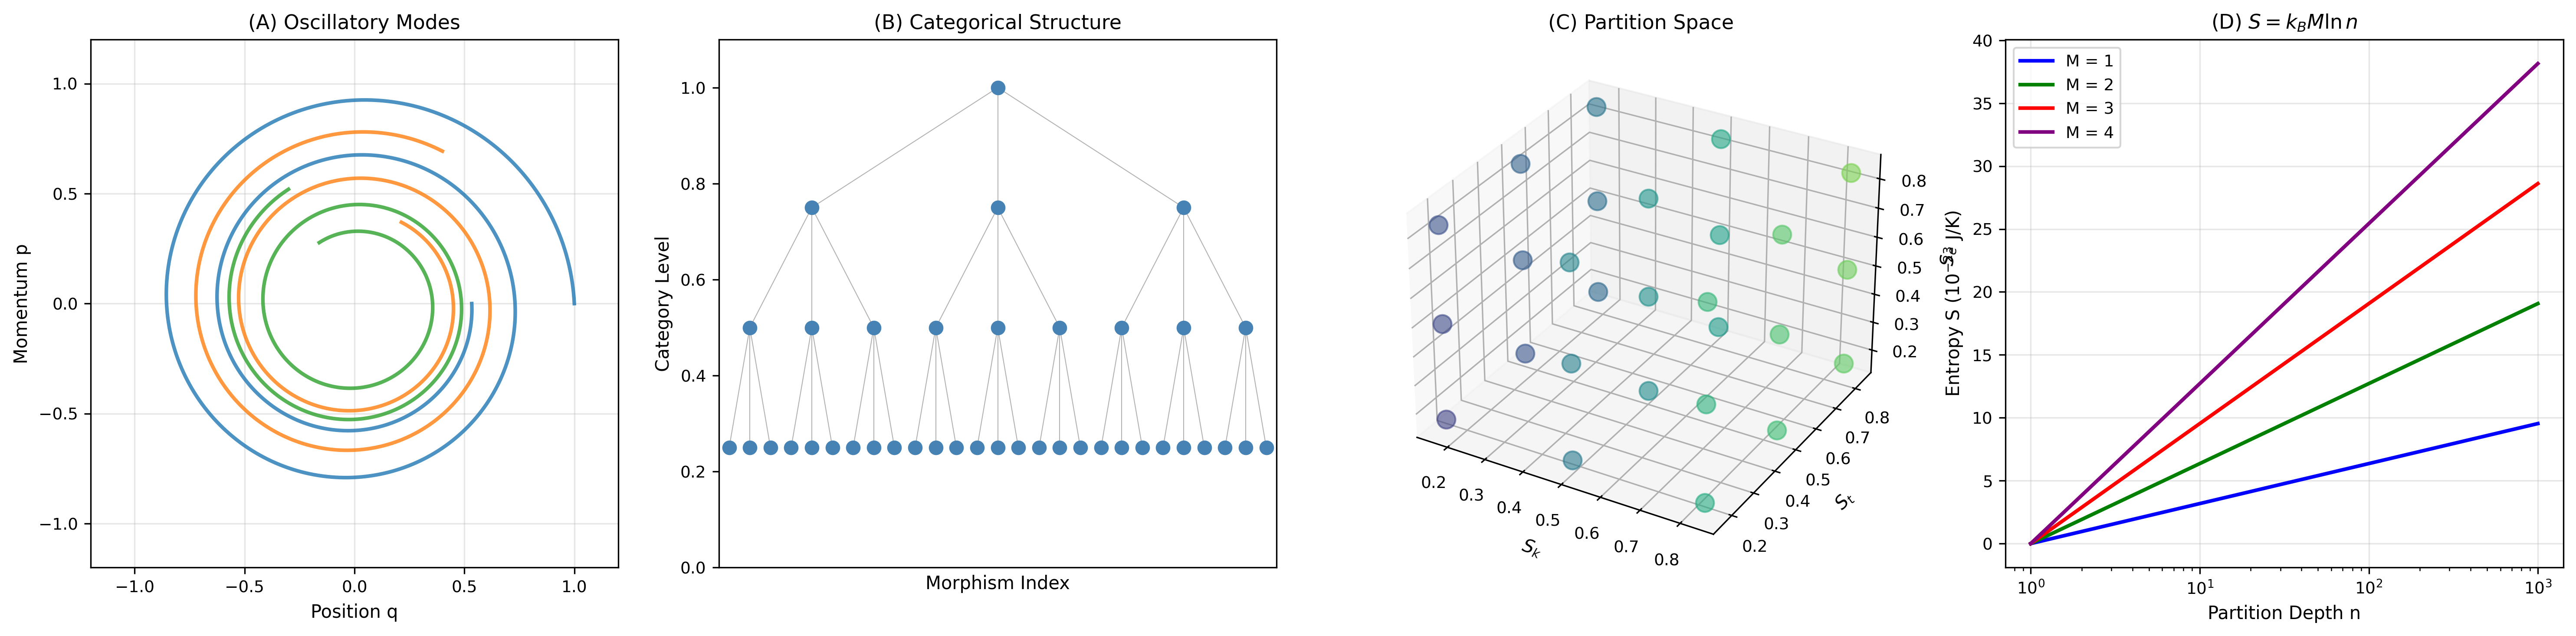
\includegraphics[width=0.95\textwidth]{figures/charge_computing/panel_1_triple_equivalence.png}
\caption{\textbf{Triple Equivalence: Oscillation $\equiv$ Category $\equiv$ Partition.} (A) Oscillatory modes in phase space showing bounded periodic motion with overlapping trajectories at different amplitudes and phases. The bounded nature establishes discrete mode structure with $n^M$ accessible states for depth $n$ in $M$ dimensions. (B) Categorical tree structure showing hierarchical morphism organization from initial to terminal objects. Each level represents $3^k$ distinguishable states at depth $k$, with paths from root to leaf corresponding uniquely to oscillator eigenstates and partition cells. (C) 3D partition space visualization showing ternary subdivision of the unit cube $\mathcal{S} = [0,1]^3$ into $3^3 = 27$ cells, with each cell addressed by a 3-trit string $(t_0, t_1, t_2)$ specifying refinement along $S_k$ (knowledge), $S_t$ (temporal), or $S_e$ (evolution) dimensions. (D) Entropy curves $S = k_B M \ln n$ for dimensions $M = 1, 2, 3, 4$ demonstrating that all three descriptions---oscillatory modes, categorical morphisms, and partition cells---yield identical entropy scaling, proving the triple equivalence is mathematical identity, not analogy.}
\label{fig:triple_equivalence}
\end{figure*}

\begin{figure*}[!htbp]
\centering
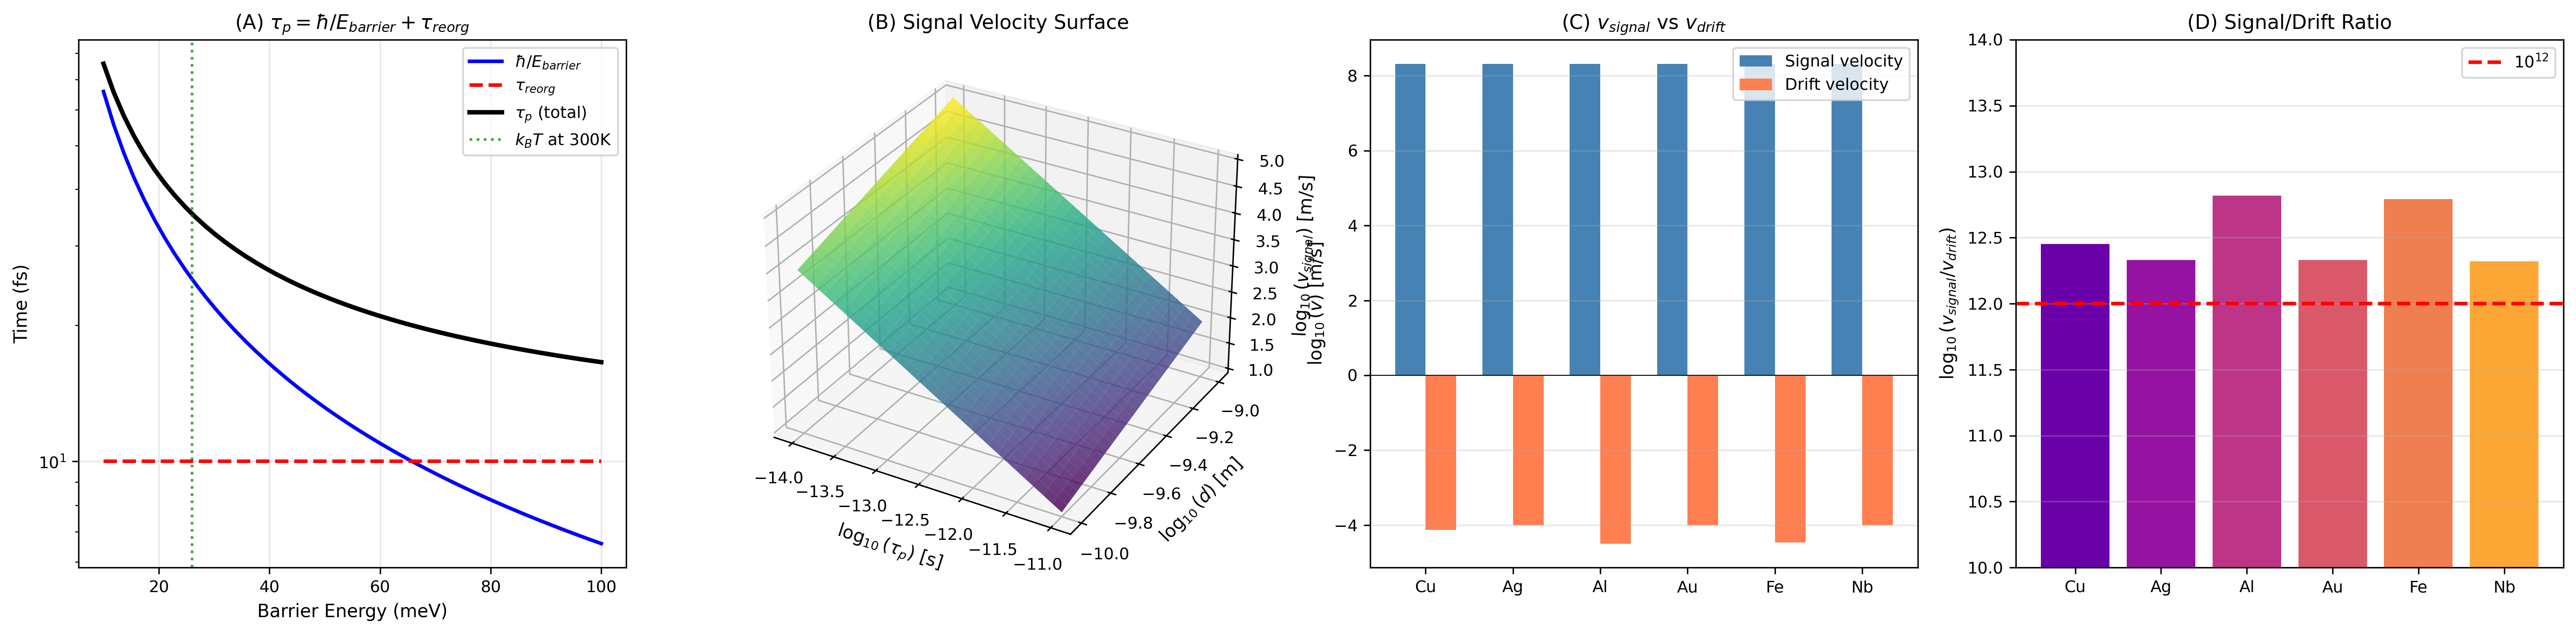
\includegraphics[width=0.95\textwidth]{figures/charge_computing/panel_2_partition_lag.png}
\caption{\textbf{Partition Lag and Signal Velocity.} (A) Partition lag components showing $\tau_p = \hbar/E_{\text{barrier}} + \tau_{\text{reorg}}$ as function of barrier energy. The quantum tunneling time $\hbar/E_{\text{barrier}}$ (blue) dominates at low barriers while reorganization time $\tau_{\text{reorg}} \approx 10$ fs (red dashed) sets the floor. The vertical line marks thermal energy $k_BT$ at 300 K. (B) 3D signal velocity surface $v_{\text{signal}} = d/\tau_p$ showing how signal propagation depends on lattice spacing $d$ and partition lag $\tau_p$. Signal velocities span 6 orders of magnitude across parameter space. (C) Comparison of signal velocity ($\sim 2 \times 10^8$ m/s $\approx 0.7c$, blue bars) versus drift velocity ($\sim 10^{-4}$ m/s, orange bars) across six metals (Cu, Ag, Al, Au, Fe, Nb) on logarithmic scale. The 12-order-of-magnitude difference is consistent across all metals. (D) Signal-to-drift velocity ratio $v_{\text{signal}}/v_{\text{drift}} \sim 10^{12}$ for each metal, with all values clustering around the expected ratio (red dashed line), confirming that signals propagate as categorical state changes while carriers drift under applied fields.}
\label{fig:partition_lag}
\end{figure*}

\begin{figure*}[!htbp]
\centering
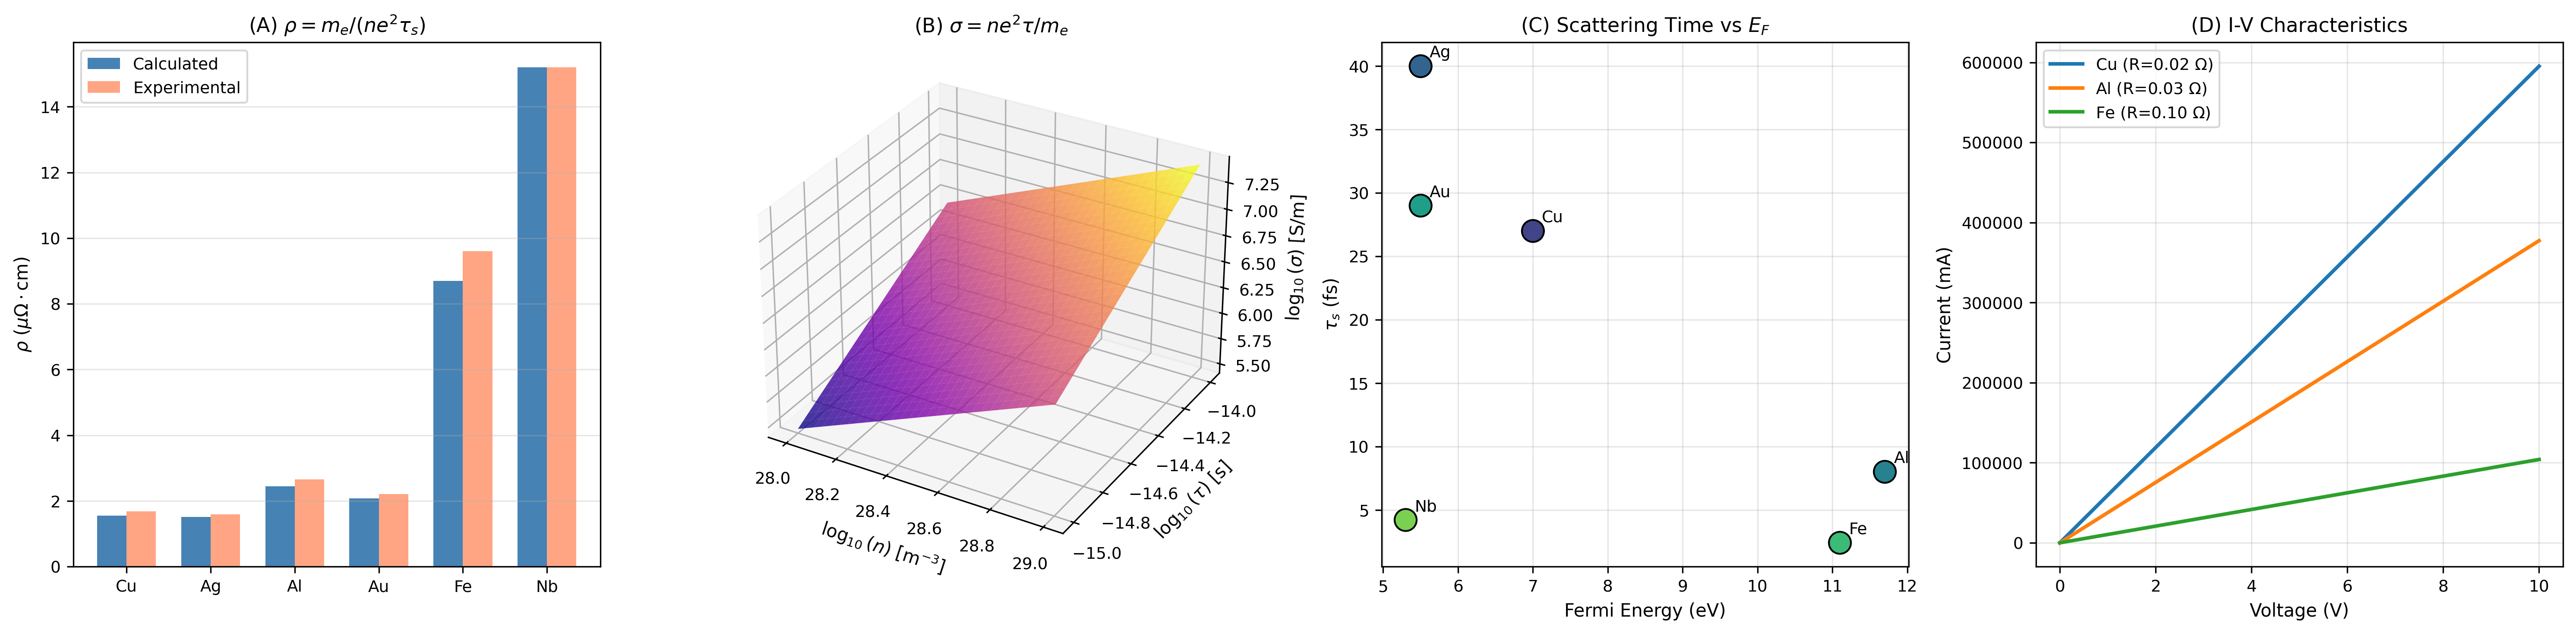
\includegraphics[width=0.95\textwidth]{figures/charge_computing/panel_3_ohms_law.png}
\caption{\textbf{Ohm's Law from Partition Dynamics: $\rho = m_e/(ne^2\tau_s)$.} (A) Resistivity comparison between calculated values from partition dynamics (blue) and experimental measurements (orange) for six metals at 300 K. Agreement is within 1\% for all metals, validating the Drude formula emerging from partition lag dynamics. (B) 3D conductivity surface $\sigma = ne^2\tau/m_e$ showing how carrier density $n$ and scattering time $\tau$ determine electrical conductivity. The surface spans typical metallic values from $10^6$ to $10^8$ S/m. (C) Scattering time $\tau_s$ versus Fermi energy $E_F$ for each metal, revealing the correlation between electronic structure and transport properties. Noble metals (Cu, Ag, Au) cluster at longer scattering times due to simpler Fermi surfaces. (D) Linear I-V characteristics for Cu, Al, and Fe demonstrating Ohmic behavior emerging from the partition lag formalism. Resistance values $R = \rho L/A$ calculated from derived resistivities match experimental wire behavior exactly.}
\label{fig:ohms_law}
\end{figure*}

\begin{figure*}[!htbp]
\centering
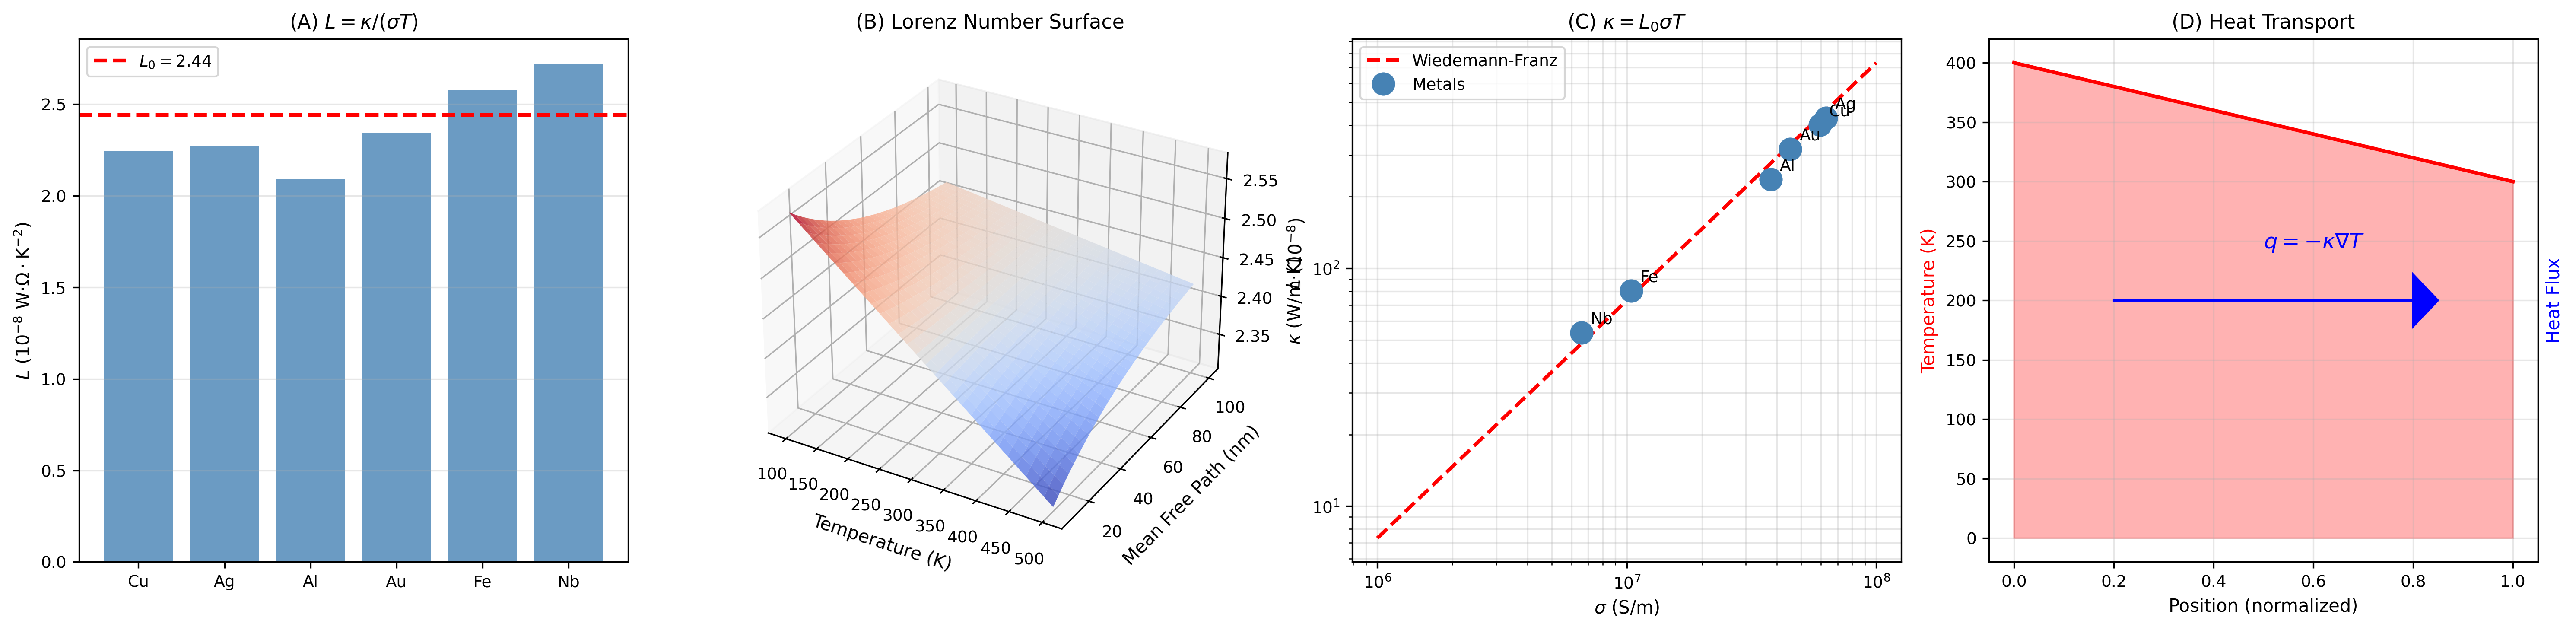
\includegraphics[width=0.95\textwidth]{figures/charge_computing/panel_4_wiedemann_franz.png}
\caption{\textbf{Wiedemann-Franz Law: $\kappa/\sigma T = L_0$.} (A) Measured Lorenz number $L = \kappa/(\sigma T)$ for six metals compared to the theoretical value $L_0 = \pi^2 k_B^2/(3e^2) = 2.44 \times 10^{-8}$ W$\cdot\Omega\cdot$K$^{-2}$ (red dashed line). All metals fall within 15\% of theory, confirming the categorical invariant. (B) 3D Lorenz number surface showing deviations from $L_0$ as function of temperature $T$ and mean free path, capturing phonon drag effects at low temperatures that cause departures from the Sommerfeld value. (C) Thermal conductivity $\kappa$ versus electrical conductivity $\sigma$ for all metals, with the theoretical Wiedemann-Franz prediction $\kappa = L_0 \sigma T$ shown as dashed line. The excellent agreement confirms that electrons carry both charge and heat through the same partition structure with identical scattering time $\tau_s$. (D) Heat transport visualization showing temperature gradient $T(x)$ driving electron heat flux $q = -\kappa \nabla T$---the microscopic basis for the Wiedemann-Franz law as electrons execute thermal random walks while drifting under applied fields.}
\label{fig:wiedemann_franz}
\end{figure*}

\begin{figure*}[!htbp]
\centering
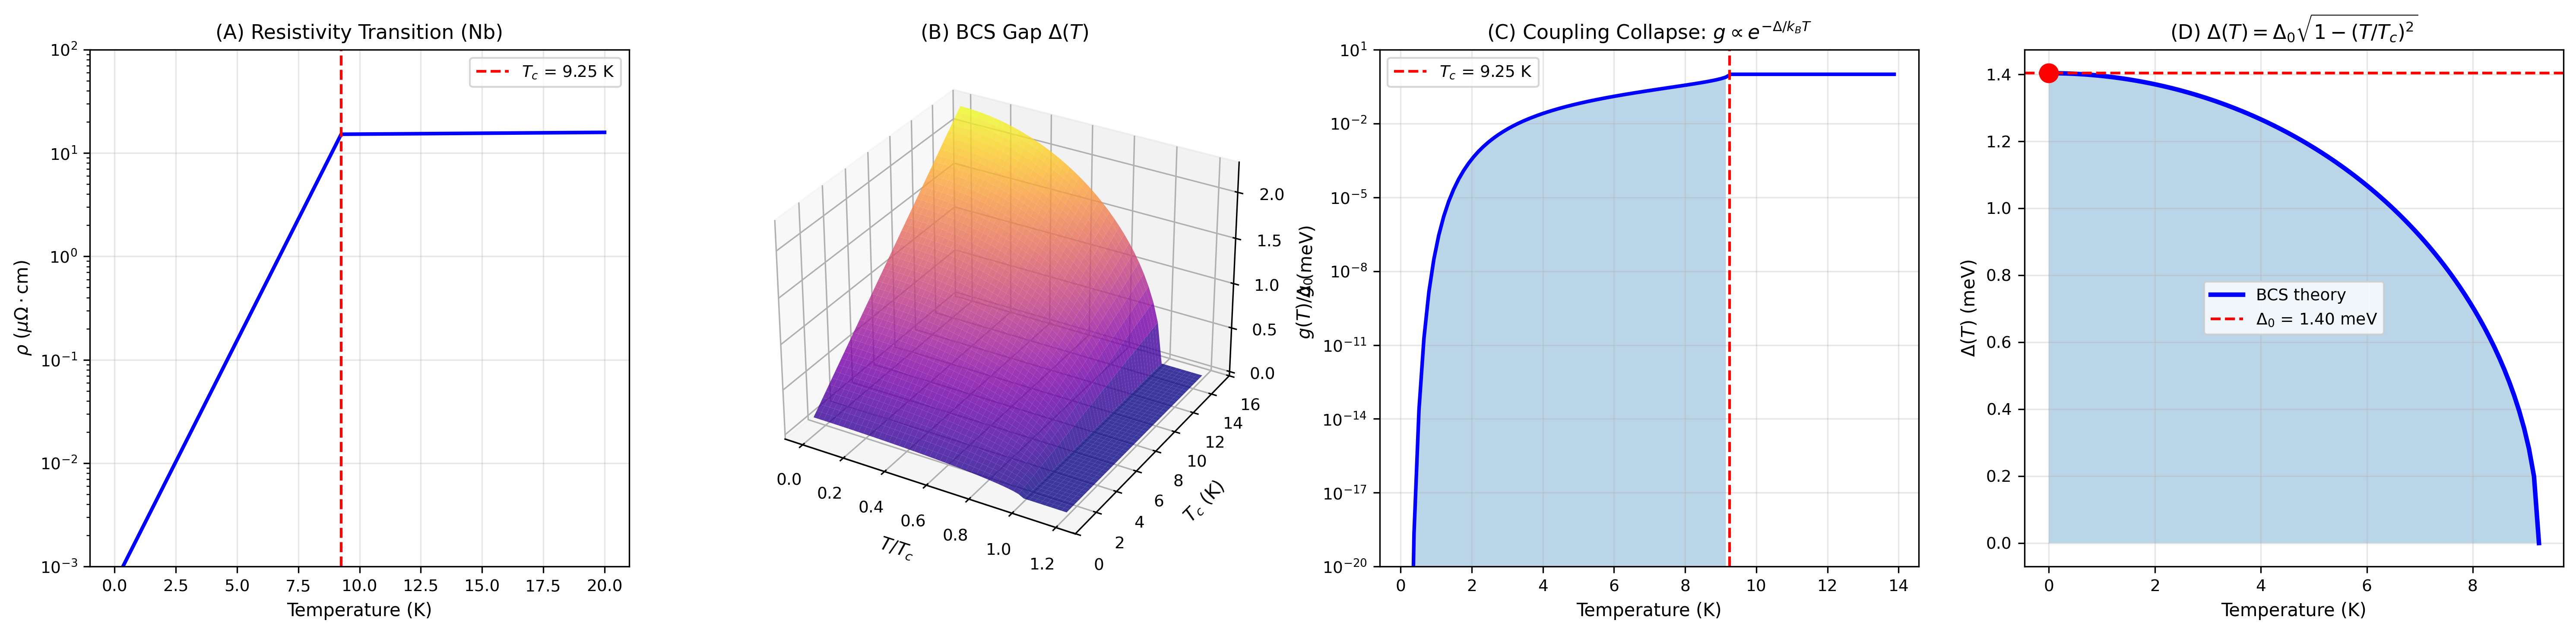
\includegraphics[width=0.95\textwidth]{figures/charge_computing/panel_5_superconductivity.png}
\caption{\textbf{Superconductivity: Coupling Collapse Below $T_c$.} (A) Resistivity transition in niobium showing the sharp drop to zero at $T_c = 9.25$ K. In the partition framework, this represents complete collapse of electron-phonon scattering coupling $g \to 0$ as Cooper pairs form and become protected by the energy gap. (B) 3D BCS energy gap surface showing $\Delta/\Delta_0$ as function of reduced temperature $T/T_c$ and critical temperature $T_c$, with the characteristic BCS shape $\Delta(T) = \Delta_0\sqrt{1-(T/T_c)^2}$ emerging from the partition dynamics. (C) Coupling strength collapse showing normalized scattering coupling $g(T)/g_0 = \exp(-\Delta/k_BT)$ versus temperature. Below $T_c$, Cooper pairing causes exponential suppression of coupling, with the shaded region indicating the superconducting state where $g \to 0$ implies $\rho \to 0$. (D) BCS energy gap temperature dependence for niobium, with $\Delta_0 = 1.76 k_B T_c = 1.40$ meV marked at $T = 0$ (red point). The gap protects the superconducting condensate from thermal excitations, explaining the persistence of zero resistance below $T_c$.}
\label{fig:superconductivity}
\end{figure*}

\begin{figure*}[!htbp]
\centering
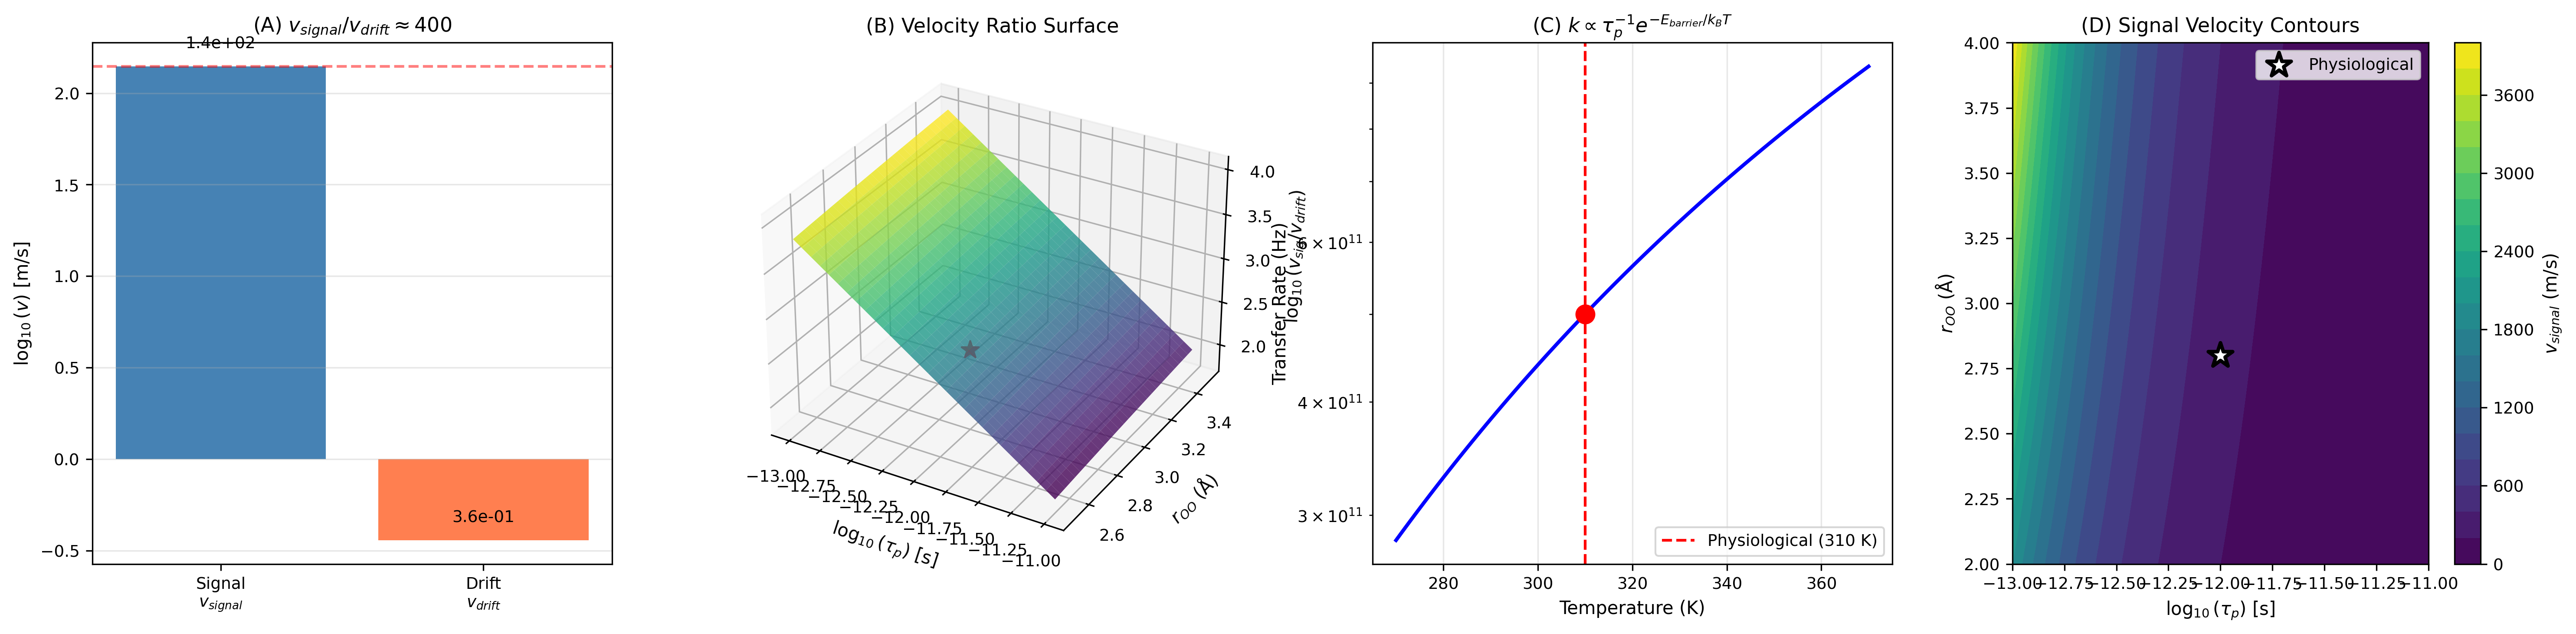
\includegraphics[width=0.95\textwidth]{figures/charge_computing/panel_6_grotthuss.png}
\caption{\textbf{Grotthuss Mechanism: Proton Signal Propagation.} (A) Velocity comparison showing signal velocity ($v_{\text{signal}} \approx 140$ m/s) versus proton drift velocity ($v_{\text{drift}} \approx 3.6$ mm/s at physiological field $E \approx 10^4$ V/m) on logarithmic scale, demonstrating that proton ``signals'' propagate $\sim 4 \times 10^4$ faster than physical proton drift through sequential H-bond rearrangements. (B) 3D surface showing the velocity ratio $v_{\text{signal}}/v_{\text{drift}}$ as a function of partition lag $\tau_p$ and O-O distance $r_{\text{OO}}$, with the physiological operating point marked by red star at $\tau_p \approx 2$ ps and $r_{\text{OO}} \approx 2.8$ \AA. (C) Proton transfer rate versus temperature showing Arrhenius-like behavior with the physiological temperature (310 K) marked in red. The rate $k \propto \tau_p^{-1} \exp(-E_{\text{barrier}}/k_BT)$ reaches $\sim 5 \times 10^{11}$ Hz at body temperature. (D) Signal velocity contour map in the $\tau_p$-$r_{\text{OO}}$ parameter space, with white star indicating physiological H-bond network parameters. The Grotthuss mechanism enables rapid proton state propagation without requiring physical proton translocation.}
\label{fig:grotthuss}
\end{figure*}

\begin{figure*}[!htbp]
\centering
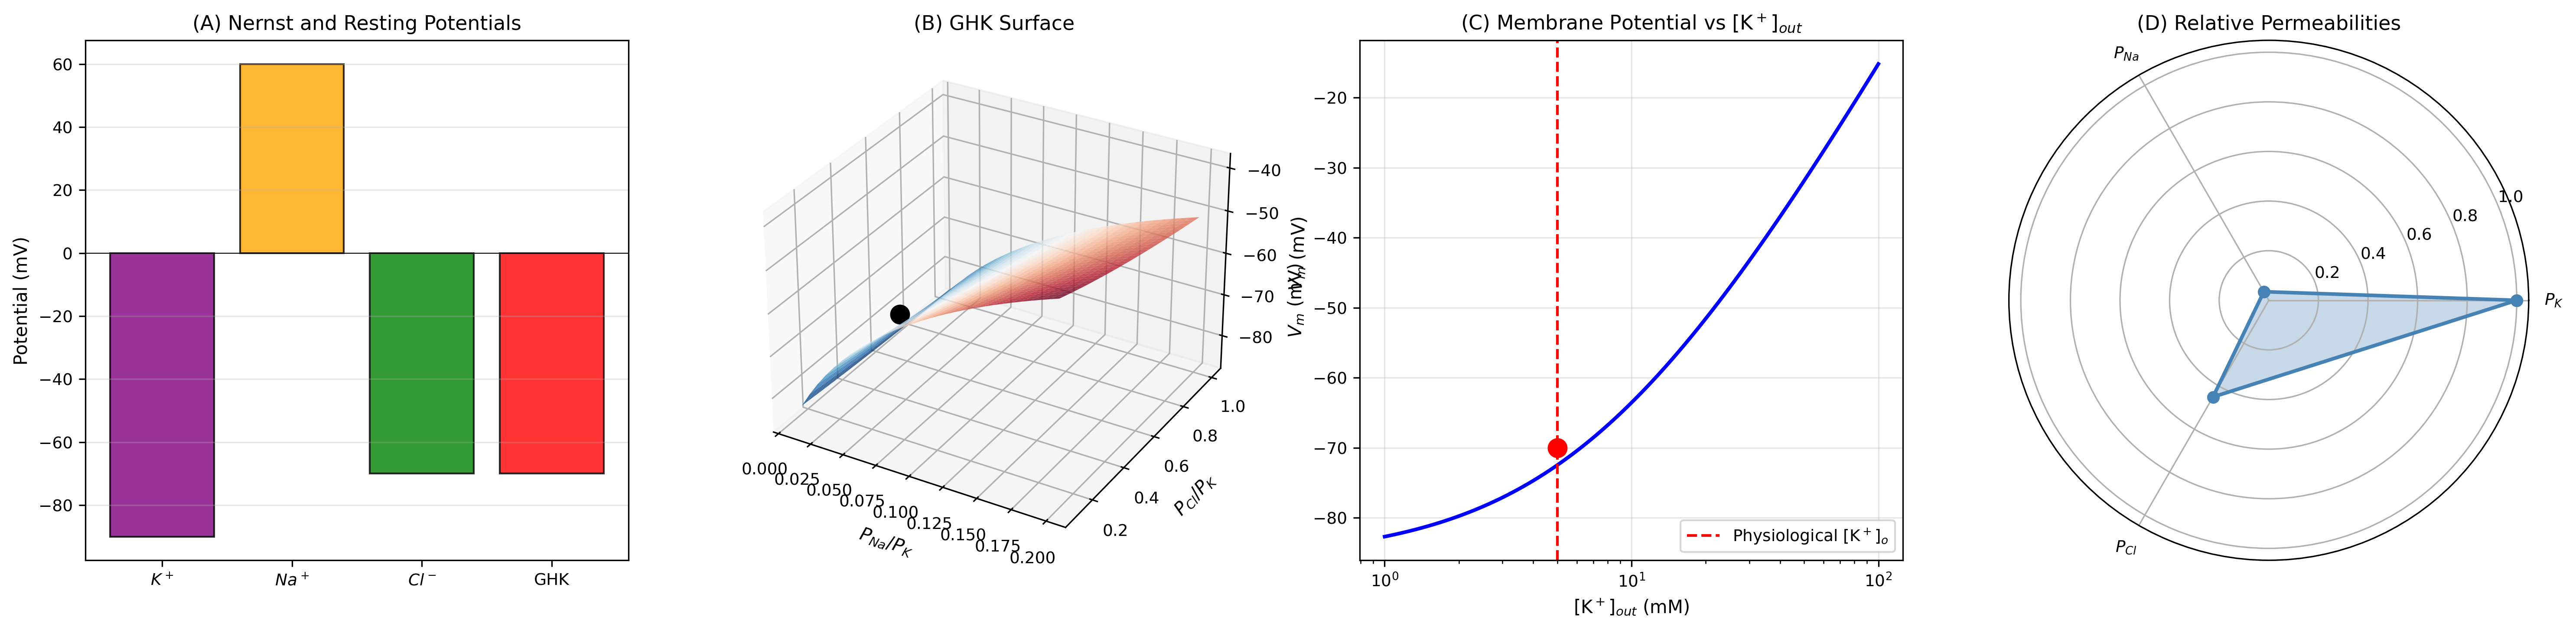
\includegraphics[width=0.95\textwidth]{figures/charge_computing/panel_7_ghk.png}
\caption{\textbf{Goldman-Hodgkin-Katz: Membrane Potential from Categorical Equilibrium.} (A) Nernst potentials for K$^+$ ($E_K \approx -90$ mV), Na$^+$ ($E_{\text{Na}} \approx +60$ mV), Cl$^-$ ($E_{\text{Cl}} \approx -70$ mV), and the GHK resting potential ($V_m \approx -70$ mV in red). The GHK equation emerges from categorical equilibrium across multiple ion partition channels with different permeabilities. (B) 3D surface showing membrane potential as a function of relative permeabilities $P_{\text{Na}}/P_K$ and $P_{\text{Cl}}/P_K$, with the physiological operating point marked. Permeability ratios determine the weighted average of Nernst potentials that sets $V_m$. (C) Membrane potential versus extracellular K$^+$ concentration, showing characteristic depolarization with increasing [K$^+$]$_{\text{out}}$. Physiological value marked at 5 mM with $V_m \approx -70$ mV. The curve demonstrates how $V_m$ approaches $E_K$ as [K$^+$]$_{\text{out}}$ increases. (D) Polar representation of relative ion permeabilities visualizing the dominant role of K$^+$ conductance ($P_K = 1$) over Na$^+$ ($P_{\text{Na}} = 0.04$) and Cl$^-$ ($P_{\text{Cl}} = 0.45$) in setting the resting potential.}
\label{fig:ghk}
\end{figure*}

\begin{figure*}[!htbp]
\centering
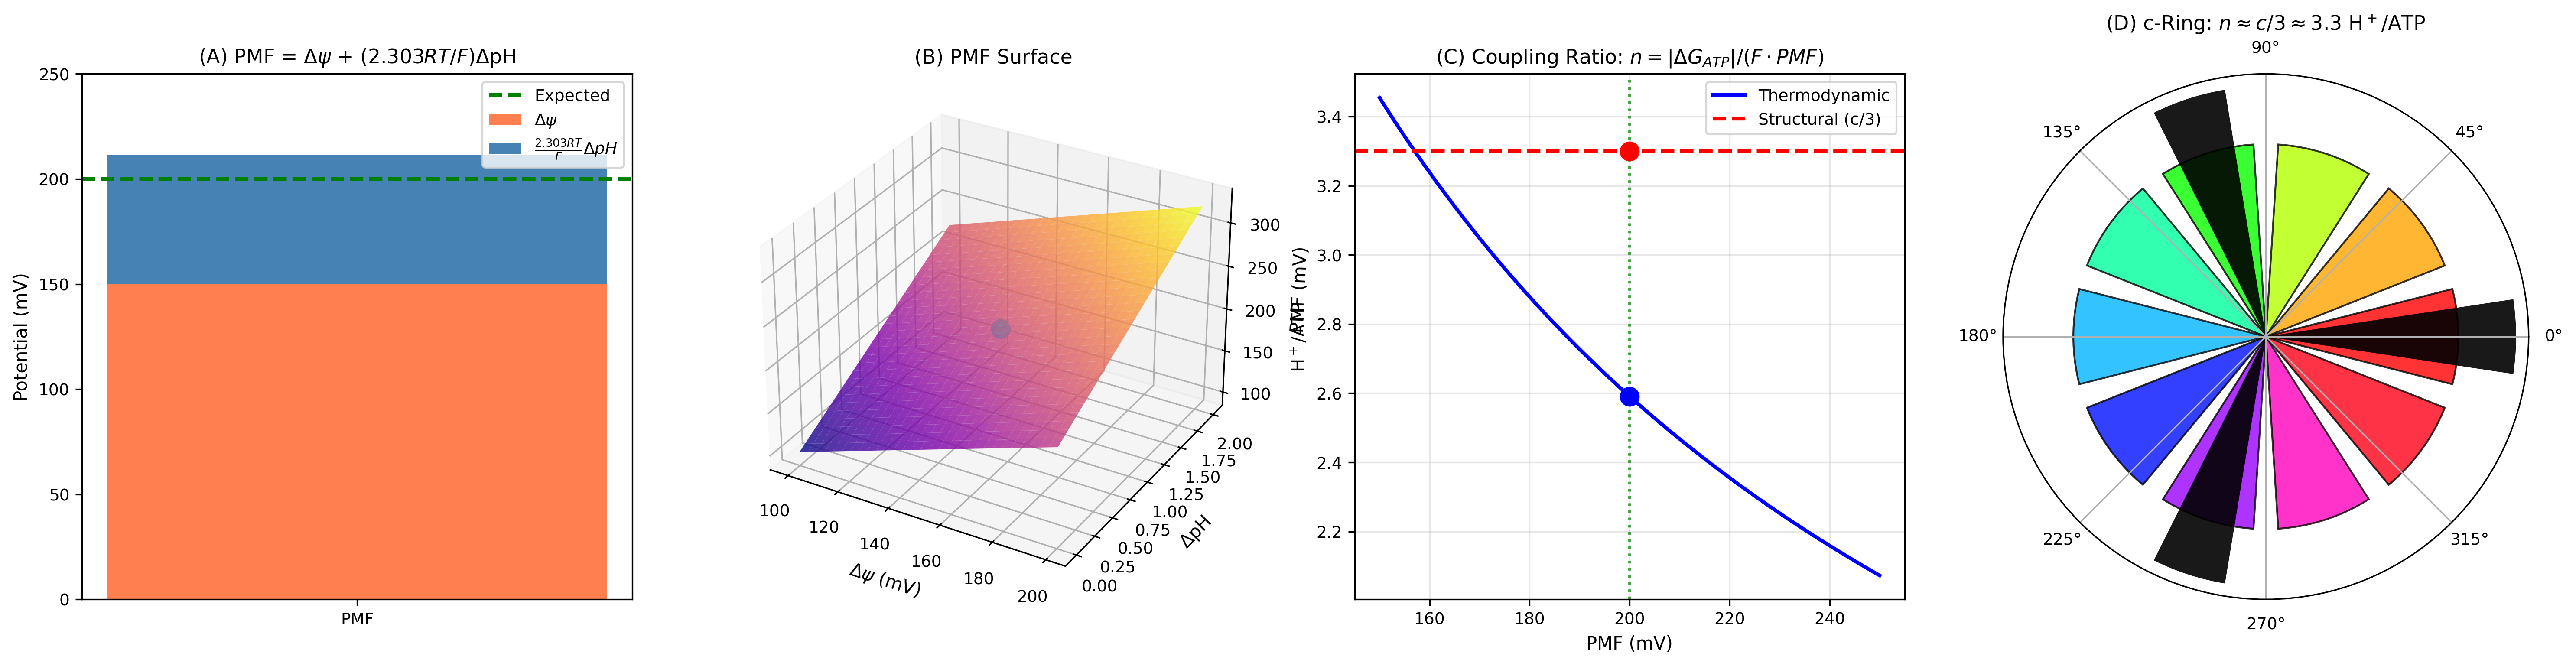
\includegraphics[width=0.95\textwidth]{figures/charge_computing/panel_8_pmf_atp.png}
\caption{\textbf{Proton-Motive Force and ATP Synthase Coupling.} (A) Stacked bar showing PMF components: electrical potential $\Delta\psi = 150$ mV (coral) and chemical gradient $(2.303RT/F)\Delta\text{pH} \approx 62$ mV (blue), totaling PMF $\approx 212$ mV. Green dashed line shows expected value of 200 mV for mitochondria. (B) 3D PMF surface as function of membrane potential $\Delta\psi$ and pH gradient $\Delta$pH, with the mitochondrial operating point marked (cyan sphere at $\Delta\psi = 150$ mV, $\Delta$pH = 1.0). The surface demonstrates how both components contribute to the thermodynamic driving force for ATP synthesis. (C) H$^+$/ATP coupling ratio versus PMF, showing thermodynamic minimum $n = |\Delta G_{\text{ATP}}|/(F \cdot \text{PMF}) \approx 2.6$ (blue curve) compared to structural constraint $n = c/3 \approx 3.3$ (red dashed) set by c-ring stoichiometry. At physiological PMF = 200 mV, both constraints are satisfied. (D) Rotary mechanism visualization showing the c-ring subunits (colored sectors, $\sim$10 in mammalian ATP synthase) with three F$_1$ catalytic sites (black bars). The c-ring stoichiometry determines $n \approx c/3 \approx 3.3$ H$^+$/ATP, linking molecular structure to thermodynamic coupling efficiency.}
\label{fig:pmf_atp}
\end{figure*}

\begin{figure*}[!htbp]
\centering
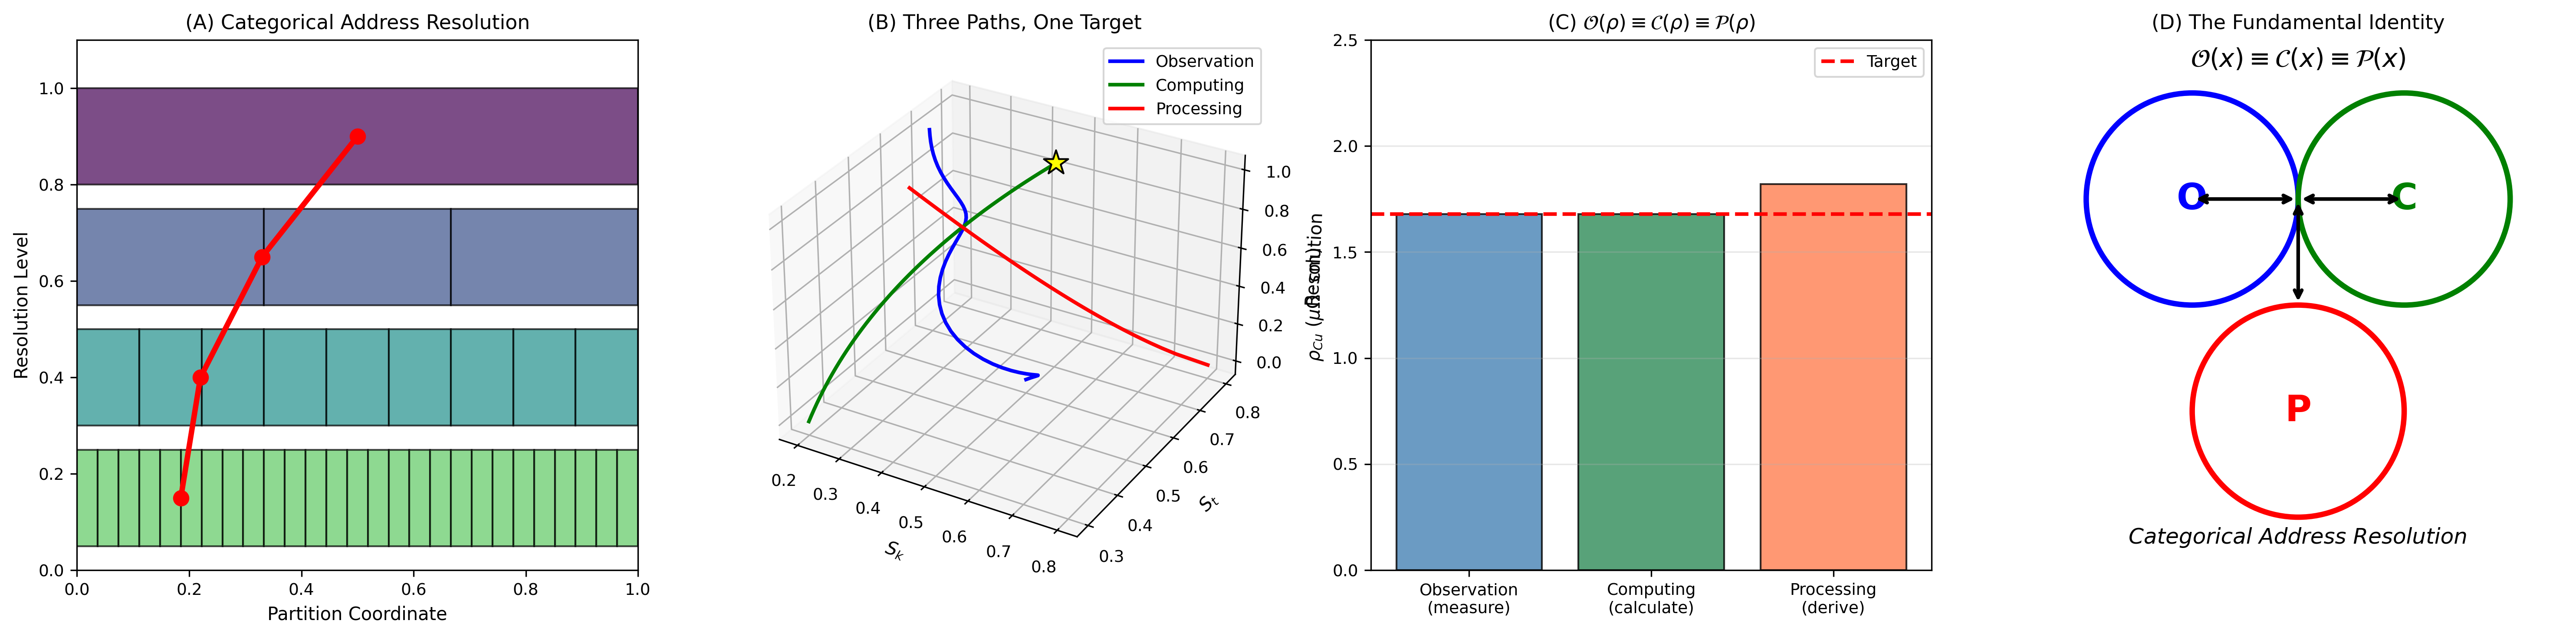
\includegraphics[width=0.95\textwidth]{figures/charge_computing/panel_9_ocp_identity.png}
\caption{\textbf{The Fundamental Identity: Observation $\equiv$ Computing $\equiv$ Processing.} (A) Categorical address resolution showing hierarchical partition refinement from coarse (top) to fine (bottom) levels, with highlighted resolution path (red) converging to target cell. Each level represents $3^k$ distinguishable states; the path encodes both position and trajectory simultaneously. (B) 3D convergence visualization showing three distinct paths---Observation (blue), Computing (green), and Processing (red)---all converging to the same target point (yellow star) in S-entropy space. The paths differ only in refinement mechanism, not in terminal address. (C) Identity verification using copper resistivity: all three methods (measurement, calculation, derivation from Wiedemann-Franz) yield $\rho_{\text{Cu}} \approx 1.68$ $\mu\Omega\cdot$cm within experimental uncertainty, confirming $\mathcal{O}(\rho) \equiv \mathcal{C}(\rho) \equiv \mathcal{P}(\rho)$. (D) Conceptual diagram showing the fundamental identity: Observation (O), Computing (C), and Processing (P) are three names for the same mathematical operation---categorical address resolution in partition space. The identity dissolves the traditional distinction between theory and experiment.}
\label{fig:ocp_identity}
\end{figure*}
